\documentclass[
  bibliography=totoc,     % Literatur im Inhaltsverzeichnis
  captions=tableheading,  % Tabellenüberschriften
  titlepage=firstiscover, % Titelseite ist Deckblatt
]{scrartcl}

% Paket float verbessern
\usepackage{scrhack}

% Warnung, falls nochmal kompiliert werden muss
\usepackage[aux]{rerunfilecheck}

% unverzichtbare Mathe-Befehle
\usepackage{amsmath}
% viele Mathe-Symbole
\usepackage{amssymb}
% Erweiterungen für amsmath
\usepackage{mathtools}

% Fonteinstellungen
\usepackage{fontspec}
% Latin Modern Fonts werden automatisch geladen
% Alternativ zum Beispiel:
%\setromanfont{Libertinus Serif}
%\setsansfont{Libertinus Sans}
%\setmonofont{Libertinus Mono}

% Wenn man andere Schriftarten gesetzt hat,
% sollte man das Seiten-Layout neu berechnen lassen
\recalctypearea{}

% deutsche Spracheinstellungen
\usepackage{polyglossia}
\setmainlanguage{german}


\usepackage[
  math-style=ISO,    % ┐
  bold-style=ISO,    % │
  sans-style=italic, % │ ISO-Standard folgen
  nabla=upright,     % │
  partial=upright,   % ┘
  warnings-off={           % ┐
    mathtools-colon,       % │ unnötige Warnungen ausschalten
    mathtools-overbracket, % │
  },                       % ┘
]{unicode-math}

% traditionelle Fonts für Mathematik
\setmathfont{Latin Modern Math}
% Alternativ zum Beispiel:
%\setmathfont{Libertinus Math}

\setmathfont{XITS Math}[range={scr, bfscr}]
\setmathfont{XITS Math}[range={cal, bfcal}, StylisticSet=1]

% Zahlen und Einheiten
\usepackage[
  locale=DE,                   % deutsche Einstellungen
  separate-uncertainty=true,   % immer Fehler mit \pm
  per-mode=symbol-or-fraction, % / in inline math, fraction in display math
]{siunitx}

% chemische Formeln
\usepackage[
  version=4,
  math-greek=default, % ┐ mit unicode-math zusammenarbeiten
  text-greek=default, % ┘
]{mhchem}

% richtige Anführungszeichen
\usepackage[autostyle]{csquotes}

% schöne Brüche im Text
\usepackage{xfrac}

% Standardplatzierung für Floats einstellen
\usepackage{float}
\floatplacement{figure}{htbp}
\floatplacement{table}{htbp}

% Floats innerhalb einer Section halten
\usepackage[
  section, % Floats innerhalb der Section halten
  below,   % unterhalb der Section aber auf der selben Seite ist ok
]{placeins}

% Seite drehen für breite Tabellen: landscape Umgebung
\usepackage{pdflscape}

% Captions schöner machen.
\usepackage[
  labelfont=bf,        % Tabelle x: Abbildung y: ist jetzt fett
  font=small,          % Schrift etwas kleiner als Dokument
  width=0.9\textwidth, % maximale Breite einer Caption schmaler
]{caption}
% subfigure, subtable, subref
\usepackage{subcaption}

% Grafiken können eingebunden werden
\usepackage{graphicx}
% größere Variation von Dateinamen möglich
\usepackage{grffile}

% schöne Tabellen
\usepackage{booktabs}

% Verbesserungen am Schriftbild
\usepackage{microtype}

% Literaturverzeichnis
\usepackage[
  backend=biber,
]{biblatex}
% Quellendatenbank
\addbibresource{lit.bib}
\addbibresource{programme.bib}

% Hyperlinks im Dokument
\usepackage[
  unicode,        % Unicode in PDF-Attributen erlauben
  pdfusetitle,    % Titel, Autoren und Datum als PDF-Attribute
  pdfcreator={},  % ┐ PDF-Attribute säubern
  pdfproducer={}, % ┘
]{hyperref}
% erweiterte Bookmarks im PDF
\usepackage{bookmark}

% Trennung von Wörtern mit Strichen
\usepackage[shortcuts]{extdash}

\author{%
  AUTOR A\\%
  \href{mailto:authorA@udo.edu}{authorA@udo.edu}%
  \texorpdfstring{\and}{,}%
  AUTOR B\\%
  \href{mailto:authorB@udo.edu}{authorB@udo.edu}%
}
\publishers{TU Dortmund – Fakultät Physik}


\title{Versuch 101 "Das Trägheitsmoment"}

\author{
  Robert Konradi\\%
  \href{mailto:authorA@udo.edu}{robert.konradi@tu-dortmund.de}%
  \texorpdfstring{\and}{,}%
  Lauritz Klünder\\%
  \href{mailto:authorB@udo.edu}{lauritz.kluender@tu-dortmund.de}%
}
\date{Durchführung: 17.11.2017, Abgabe: 24.11.2017}
\publishers{TU Dortmund – Fakultät Physik}
\begin{document}
\maketitle
\setlength{\parindent}{0pt}
%\thispagestyle{empty}
\tableofcontents
\newpage
\section{Einleitung}
Das Trägheitsmoment von verschiedene Körpern soll bestimmt werden und der Satz von Steiner verifiziert werden.
\section{Theorie}
Das Drehmoment $M$, das Trägheitsmoment $I$ als auch die Winkelbeschleunigung \.{\omega} charakterisieren die Rotationsbewegung.
Für eine punktförmige Masse kann das Trägheitsmoment mit $I = m*r^2$ berechnen. Dabei ist m die Masse und r der Abstand zur Drehachse.
Für ein ausgedehnten Körper um eine feste Achse kann das Gesamtträgheitsmoment als:
\begin{equation}
  I=\sum \limits_{i}^{} r_\text{i}^2 \cdot m_\text{i}
\end{equation}
dargestellt werden.
Das Drehmoment $M$ ist von der Lage der Drehachse abhängig.
Für geometrische Objekte, wie ein Kugel, Stab, Zylinder, lässt sich das Trägheitsmoment
leicht bestimmen.
In Abbildung 1 sind verschiedene Objekte mit deren Trägheitsmoment dargestellt.
\begin{figure}[H]
\centering
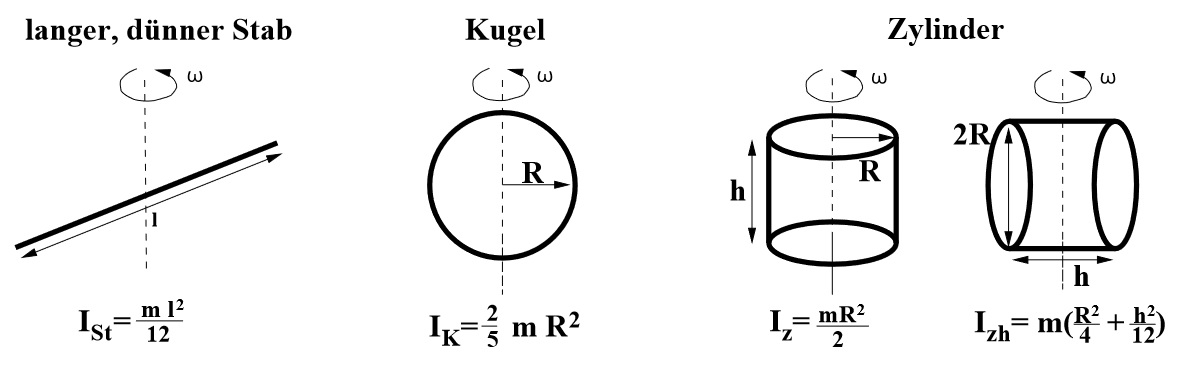
\includegraphics[width=\textwidth]{Bild1.jpg}
\caption{Objekte mit deren Trägheitsmoment}[1]
\label{fig:Abb1}
\end{figure}
Ist die Drehachse nicht durch den Schwerpunkt eines Körpers sondern parallel mit einem Abstand a
zur gehenden Achse verschoben, so lässt sich das Trägheitsmoment mithilfe von Satz des Steiners
\begin{equation}
  I = I_\text{0} + m*a^2
\end{equation}
erechnen. Dabei ist $I_\text{0}$ das Trägheitsmoment der Drehachse durch den Schwerpunkt des Körpers.
Greift eine Kraft mit einem Abstand r von der Achse auf ein drehenden Körper, so wirkt ein Drehmoment $\vec{M} = \vec{F} \times \vec{r}$.
In einem Schwingungssystem wirkt auf ein Körper durch die Drehung um ein Winkel $\phi$ aus seiner Ruhelage ein rücktreibenes Drehmoment
durch eine Feder entgegen. Die harmonische Schwingung lässt sich mit der Schwingungsdauer
\begin{equation}
  T = 2\pi \sqrt{\frac{I}{D}}
\end{equation}
berechnen. I ist dabei das Trägheitsmoment und D die Winkelrichtsgröße.
\begin{equation}
  D = \frac{M}{\phi} \leftrightarrow D = \frac{F \cdot r}{\phi}
\end{equation}
Das harmonische Verhalten bei der Drehschwingung ist nur auf kleinen Winekl $\phi$
beschränkt.

\section{Versuchsaufbau}
Zur Bestimmung des Trägheitsmoments I wird zunächst die
die Drillachse, siehe Abbildung 2, benötigt. Die Drillachse
die über eine Spiralfeder mit einem Rahmen verbunden.
\begin{figure}[H]
  \centering
  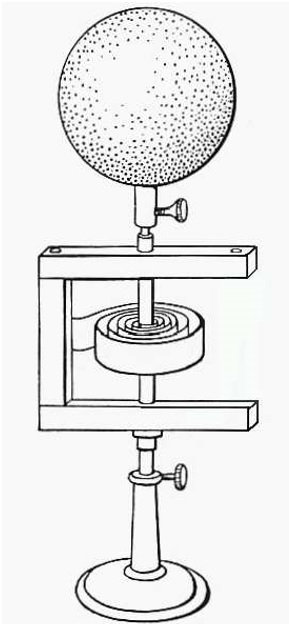
\includegraphics[width=5 cm , height= 10 cm]{Bild2.jpg}
   \caption{Schematische Darstellung des Versuchsaufbau}
\end{figure}
Auf die Achse können verschiedene Objekte angebracht werden.
%Das Eigenträgheitsmoment $I_\text{D}$ sowie die Winkelrichtgröße D lässt sich über die Schwingungsdauer T
%berechnet.

 \section{Durchführung}

\printbibliography{}
\nocite{*}
\end{document}
